% ===========================================================================
%  Sliding-Window Factor Graph Optimisation: Theory and Marginalization
%  Companion document for the SW-FGO MATLAB implementation
% ===========================================================================
\documentclass[11pt,a4paper]{article}

% --- Packages ---
\usepackage[utf8]{inputenc}
\usepackage[T1]{fontenc}
\usepackage{amsmath,amssymb,amsthm}
\usepackage{bm}
\usepackage{mathtools}
\usepackage{graphicx}
\usepackage[margin=2.5cm]{geometry}
\usepackage{hyperref}
\usepackage{cleveref}
\usepackage{algorithm}
\usepackage{algpseudocode}
\usepackage{booktabs}
\usepackage{tikz}
\usetikzlibrary{positioning, arrows.meta, calc, fit, backgrounds, decorations.pathreplacing}
\usepackage{tcolorbox}
\tcbuselibrary{theorems, skins, breakable}

% --- Custom math commands ---
\newcommand{\bx}{\bm{x}}
\newcommand{\bz}{\bm{z}}
\newcommand{\br}{\bm{r}}
\newcommand{\bb}{\bm{b}}
\newcommand{\bp}{\bm{p}}
\newcommand{\bv}{\bm{v}}
\newcommand{\bJ}{\bm{J}}
\newcommand{\bH}{\bm{H}}
\newcommand{\bI}{\bm{I}}
\newcommand{\bR}{\bm{R}}
\newcommand{\bSigma}{\bm{\Sigma}}
\newcommand{\bLambda}{\bm{\Lambda}}
\newcommand{\R}{\mathbb{R}}
\newcommand{\ie}{i.e.}
\newcommand{\eg}{e.g.}
\DeclareMathOperator{\diag}{diag}
\DeclareMathOperator{\blkdiag}{blkdiag}

% --- Theorem-like environments ---
\theoremstyle{definition}
\newtheorem{definition}{Definition}[section]
\newtheorem{remark}{Remark}[section]
\theoremstyle{plain}
\newtheorem{theorem}{Theorem}[section]
\newtheorem{proposition}{Proposition}[section]

% --- Colored boxes ---
\newtcolorbox{keybox}[1][]{
  colback=blue!5!white, colframe=blue!60!black,
  fonttitle=\bfseries, title={#1},
  breakable, enhanced
}
\newtcolorbox{warnbox}[1][]{
  colback=orange!5!white, colframe=orange!70!black,
  fonttitle=\bfseries, title={#1},
  breakable, enhanced
}
\newtcolorbox{implbox}[1][]{
  colback=green!5!white, colframe=green!50!black,
  fonttitle=\bfseries, title={#1},
  breakable, enhanced
}

% ===========================================================================
\title{\textbf{Sliding-Window Factor Graph Optimisation}\\[4pt]
       \large Theory, Marginalization, and Implementation Notes}
\author{}
\date{\today}

\begin{document}
\maketitle

\tableofcontents
\vspace{1em}

% ===========================================================================
\section{Introduction}
\label{sec:intro}

Factor graph optimisation (FGO) formulates estimation as a nonlinear
least-squares problem over a graph of variable nodes (states) and factor
nodes (constraints/measurements).  In a \emph{batch} setting we collect
\emph{all} measurements and solve one large system—this yields the
globally optimal estimate but is impractical for real-time applications
because:
\begin{enumerate}
  \item the problem grows unboundedly over time,
  \item future measurements are unavailable, and
  \item computational cost scales as $\mathcal{O}(N^3)$ per iteration in
        dense solvers (or $\mathcal{O}(N)$ for banded structure, but the
        constant is still large).
\end{enumerate}

A \textbf{sliding-window} FGO (SW-FGO) resolves these issues by
maintaining only the $W$ most recent variable nodes.  When a new node
arrives and the window is at capacity, the oldest node is \emph{marginalised
out} via the Schur complement.  The information from the evicted node is
not discarded—it is compressed into a dense \textbf{marginalisation
prior} on the remaining nodes.

% ===========================================================================
\section{Batch Factor Graph Optimisation}
\label{sec:batch}

\subsection{Problem Formulation}

Consider $N$ variable nodes
$\mathcal{X} = \{\bx_1, \bx_2, \ldots, \bx_N\}$, each $\bx_k \in \R^d$.
We define a set of factors $\{f_i\}_{i=1}^{M}$, each involving one or more
variables.  Factor $f_i$ produces a \emph{residual} $\br_i(\mathcal{X}_i)$
with associated noise covariance $\bSigma_i$, where $\mathcal{X}_i \subseteq \mathcal{X}$.

The maximum a posteriori (MAP) estimate is:
\begin{equation}
  \mathcal{X}^* = \arg\min_{\mathcal{X}} \;
    \sum_{i=1}^{M} \bigl\| \br_i(\mathcal{X}_i) \bigr\|^2_{\bSigma_i},
  \label{eq:map}
\end{equation}
where the Mahalanobis norm is
$\|\br\|^2_{\bSigma} = \br^\top \bSigma^{-1} \br$.

\subsection{Gauss--Newton Iteration}

At a linearisation point $\hat{\mathcal{X}}$, each residual is approximated
by a first-order Taylor expansion:
\begin{equation}
  \br_i(\hat{\mathcal{X}}_i + \delta\bx)
    \approx \br_i(\hat{\mathcal{X}}_i) + \bJ_i \, \delta\bx,
\end{equation}
where $\bJ_i = \partial \br_i / \partial \bx$ is the Jacobian.

\begin{definition}[Whitened Residual and Jacobian]
  Given covariance $\bSigma_i = \bm{L}_i \bm{L}_i^\top$ (Cholesky),
  the \emph{square-root information} matrix is
  $\bm{S}_i = \bm{L}_i^{-1}$, so that
  $\bSigma_i^{-1} = \bm{S}_i^\top \bm{S}_i$.
  The whitened quantities are:
  \begin{equation}
    \tilde{\br}_i = \bm{S}_i \, \br_i, \qquad
    \tilde{\bJ}_i = \bm{S}_i \, \bJ_i.
  \end{equation}
\end{definition}

Stacking all whitened residuals and Jacobians into $\tilde{\br} \in \R^m$
and $\tilde{\bJ} \in \R^{m \times n}$ (with $n = N \cdot d$), the
linearised cost is:
\begin{equation}
  \sum_i \| \tilde{\br}_i + \tilde{\bJ}_i \, \delta\bx \|^2
  = \| \tilde{\br} + \tilde{\bJ} \, \delta\bx \|^2.
  \label{eq:lin_cost}
\end{equation}

Minimising \eqref{eq:lin_cost} yields the \textbf{normal equations}:
\begin{equation}
  \boxed{
    \bH \, \delta\bx = -\bb, \qquad
    \bH = \tilde{\bJ}^\top \tilde{\bJ}, \quad
    \bb = \tilde{\bJ}^\top \tilde{\br},
  }
  \label{eq:normal}
\end{equation}
where $\bH \in \R^{n \times n}$ is the \emph{Hessian approximation}
(information matrix), and $\bb$ is the \emph{information vector}.

We update $\hat{\bx} \leftarrow \hat{\bx} + \delta\bx$ and repeat until
convergence.

\subsection{Structure of the Hessian}

For a Markov chain (sequential dynamics + measurements), the Hessian is
\textbf{block-tridiagonal}:
\begin{equation}
  \bH = \begin{bmatrix}
    \bH_{11} & \bH_{12} & & \\
    \bH_{21} & \bH_{22} & \bH_{23} & \\
    & \ddots & \ddots & \ddots \\
    & & \bH_{N-1,N} & \bH_{NN}
  \end{bmatrix},
  \label{eq:H_banded}
\end{equation}
where $\bH_{kk} \in \R^{d \times d}$ accumulates all factors involving
node $k$, and $\bH_{k,k+1}$ comes from the dynamics factor linking $k \to k+1$.

\begin{remark}
  Measurements that only touch a single node (\eg{} radar, camera) contribute
  to the block-diagonal $\bH_{kk}$ only.  The between-factor (dynamics)
  creates the off-diagonal blocks $\bH_{k,k+1}$.
\end{remark}

\subsection{Marginal Covariance}

After convergence, the marginal covariance of node $k$ is the $d \times d$
block of the Hessian inverse:
\begin{equation}
  \bSigma_k = \bigl[\bH^{-1}\bigr]_{kk}.
  \label{eq:marginal_cov}
\end{equation}

% ===========================================================================
\section{The Sliding-Window Approach}
\label{sec:sliding_window}

\subsection{Motivation}

In a batch FGO with $N$ nodes, the Hessian $\bH \in \R^{Nd \times Nd}$
grows with the mission duration.  Even exploiting sparsity, memory and solve
time grow at least linearly in $N$.

The sliding-window idea is simple:

\begin{keybox}[Sliding-Window Principle]
  Maintain only the most recent $W$ variable nodes.
  When a new node $\bx_{k+1}$ arrives:
  \begin{enumerate}
    \item \textbf{Marginalise} the oldest node $\bx_{k-W+1}$ out of the
          window, producing a dense prior on the remaining $W-1$ nodes.
    \item \textbf{Add} the new node $\bx_{k+1}$ to the window (now
          $W$ nodes again).
    \item \textbf{Add} new factors (dynamics, measurements).
    \item \textbf{Optimise} the $W$-node sub-problem via Gauss--Newton.
  \end{enumerate}
\end{keybox}

The key ingredient is the \textbf{marginalization step}, which we now derive
in detail.

\subsection{Full Window at Time $k$}

At time $k$, the window contains nodes
$\mathcal{W}_k = \{\bx_{k-W+1},\, \ldots,\, \bx_k\}$.
The cost function involves:
\begin{itemize}
  \item the \textbf{marginalisation prior} from the previous window
        (encoding history for $t < k-W+1$),
  \item all dynamics factors within the window,
  \item all measurement factors with keys inside the window.
\end{itemize}

After Gauss--Newton converges, we have the linearised information at the
current estimates:
\begin{equation}
  \bH_{\text{win}} = \tilde{\bJ}^\top \tilde{\bJ}, \qquad
  \bb_{\text{win}} = -\tilde{\bJ}^\top \tilde{\br}.
  \label{eq:H_window}
\end{equation}

% ===========================================================================
\section{Marginalization via the Schur Complement}
\label{sec:marginalization}

This section is the core of the sliding-window method.  We derive
marginalization from first principles.

\subsection{Partitioning the Information System}

Suppose the window contains $W$ nodes.  We want to \textbf{eliminate node $a$}
(the oldest, slot~1) and keep nodes $b$ (slots $2, \ldots, W$).
Partition the stacked state vector as:
\begin{equation}
  \delta\bx = \begin{bmatrix} \delta\bx_a \\ \delta\bx_b \end{bmatrix},
  \qquad
  \delta\bx_a \in \R^{d}, \quad
  \delta\bx_b \in \R^{(W-1)d}.
\end{equation}

The Hessian and information vector partition correspondingly:
\begin{equation}
  \bH = \begin{bmatrix}
    \bH_{aa} & \bH_{ab} \\
    \bH_{ba} & \bH_{bb}
  \end{bmatrix}, \qquad
  \bb = \begin{bmatrix} \bb_a \\ \bb_b \end{bmatrix}.
  \label{eq:partition}
\end{equation}

The linearised cost from \eqref{eq:normal} is:
\begin{equation}
  C(\delta\bx_a, \delta\bx_b) =
    \frac{1}{2}
    \begin{bmatrix} \delta\bx_a \\ \delta\bx_b \end{bmatrix}^\top
    \begin{bmatrix} \bH_{aa} & \bH_{ab} \\ \bH_{ba} & \bH_{bb} \end{bmatrix}
    \begin{bmatrix} \delta\bx_a \\ \delta\bx_b \end{bmatrix}
    + \begin{bmatrix} \bb_a \\ \bb_b \end{bmatrix}^\top
    \begin{bmatrix} \delta\bx_a \\ \delta\bx_b \end{bmatrix}
    + c_0.
  \label{eq:quadratic_cost}
\end{equation}

\subsection{Eliminating $\delta\bx_a$ by Completing the Square}

To eliminate $\delta\bx_a$, we minimise $C$ with respect to $\delta\bx_a$
while keeping $\delta\bx_b$ fixed.  Setting
$\partial C / \partial (\delta\bx_a) = 0$:
\begin{equation}
  \bH_{aa}\,\delta\bx_a^* + \bH_{ab}\,\delta\bx_b + \bb_a = 0,
\end{equation}
which gives the optimal $\delta\bx_a$ as a function of $\delta\bx_b$:
\begin{equation}
  \boxed{
    \delta\bx_a^*(\delta\bx_b) =
      -\bH_{aa}^{-1}\bigl(\bH_{ab}\,\delta\bx_b + \bb_a\bigr).
  }
  \label{eq:xa_star}
\end{equation}

\begin{remark}
  $\bH_{aa}$ is a $d \times d$ matrix (e.g.\ $6 \times 6$ for
  position--velocity state).  Its inversion is cheap and always
  well-conditioned as long as the prior or at least one measurement
  touches node $a$.
\end{remark}

Substituting \eqref{eq:xa_star} back into \eqref{eq:quadratic_cost}
and simplifying, we obtain the \textbf{marginalised cost}—a
function of $\delta\bx_b$ only:

\begin{keybox}[Schur complement result]
\begin{align}
  C_{\text{marg}}(\delta\bx_b) &=
    \frac{1}{2}\,\delta\bx_b^\top \bH_{\text{marg}}\,\delta\bx_b
    + \bb_{\text{marg}}^\top \delta\bx_b + c_{\text{marg}},
  \label{eq:marg_cost}
\end{align}
where the \textbf{Schur complement} quantities are:
\begin{align}
  \bH_{\text{marg}} &= \bH_{bb} - \bH_{ba}\,\bH_{aa}^{-1}\,\bH_{ab},
  \label{eq:H_schur} \\[4pt]
  \bb_{\text{marg}} &= \bb_b - \bH_{ba}\,\bH_{aa}^{-1}\,\bb_a.
  \label{eq:b_schur}
\end{align}
\end{keybox}

\begin{remark}
  $\bH_{\text{marg}}$ is the \emph{Schur complement} of $\bH_{aa}$ in $\bH$.
  It is guaranteed to be positive semi-definite if $\bH$ is positive
  semi-definite (and positive definite if $\bH$ is positive definite).
\end{remark}

\subsection{Detailed Derivation of the Schur Complement}
\label{sec:schur_detail}

\paragraph{Step 1:} Expand the quadratic form in \eqref{eq:quadratic_cost}:
\begin{align}
  2C &= \delta\bx_a^\top \bH_{aa}\,\delta\bx_a
       + \delta\bx_a^\top \bH_{ab}\,\delta\bx_b
       + \delta\bx_b^\top \bH_{ba}\,\delta\bx_a
       + \delta\bx_b^\top \bH_{bb}\,\delta\bx_b \notag \\
     &\quad + 2\bb_a^\top \delta\bx_a
       + 2\bb_b^\top \delta\bx_b + 2c_0.
  \label{eq:expand_C}
\end{align}

\paragraph{Step 2:} Group terms involving $\delta\bx_a$ and
\emph{complete the square}.  Define
$\bm{g}_a = \bH_{ab}\,\delta\bx_b + \bb_a$.
The $\delta\bx_a$-dependent portion of \eqref{eq:expand_C} is:
\begin{align}
  &\delta\bx_a^\top \bH_{aa}\,\delta\bx_a
    + 2\bm{g}_a^\top \delta\bx_a \notag \\
  &= \bigl(\delta\bx_a + \bH_{aa}^{-1}\bm{g}_a\bigr)^\top
     \bH_{aa}
     \bigl(\delta\bx_a + \bH_{aa}^{-1}\bm{g}_a\bigr)
     - \bm{g}_a^\top \bH_{aa}^{-1} \bm{g}_a.
  \label{eq:complete_sq}
\end{align}

The first term in \eqref{eq:complete_sq} is always $\ge 0$ (since
$\bH_{aa} \succ 0$) and is minimised to zero when
$\delta\bx_a = -\bH_{aa}^{-1}\bm{g}_a = \delta\bx_a^*$,
recovering \eqref{eq:xa_star}.

\paragraph{Step 3:} Substitute back.  The minimum over $\delta\bx_a$ leaves:
\begin{align}
  2C_{\text{marg}} &= \delta\bx_b^\top \bH_{bb}\, \delta\bx_b
    + 2\bb_b^\top \delta\bx_b
    - \bm{g}_a^\top \bH_{aa}^{-1}\bm{g}_a + 2c_0.
\end{align}

Expand $\bm{g}_a^\top \bH_{aa}^{-1}\bm{g}_a$:
\begin{align}
  \bm{g}_a^\top \bH_{aa}^{-1}\bm{g}_a
    &= (\bH_{ab}\,\delta\bx_b + \bb_a)^\top
       \bH_{aa}^{-1}
       (\bH_{ab}\,\delta\bx_b + \bb_a) \notag \\
    &= \delta\bx_b^\top \bH_{ba}\,\bH_{aa}^{-1}\,\bH_{ab}\,\delta\bx_b
       + 2\bb_a^\top \bH_{aa}^{-1}\bH_{ab}\,\delta\bx_b
       + \bb_a^\top \bH_{aa}^{-1}\bb_a.
\end{align}

\paragraph{Step 4:} Collecting terms quadratic and linear in $\delta\bx_b$:
\begin{align}
  2C_{\text{marg}} &= \delta\bx_b^\top
    \underbrace{\bigl(\bH_{bb} - \bH_{ba}\,\bH_{aa}^{-1}\,\bH_{ab}\bigr)}_{\bH_{\text{marg}}}
    \delta\bx_b \notag \\
    &\quad + 2\underbrace{\bigl(\bb_b - \bH_{ba}\,\bH_{aa}^{-1}\bb_a\bigr)^\top}_{\bb_{\text{marg}}^\top}
    \delta\bx_b + \text{const.}
\end{align}

This confirms \eqref{eq:H_schur}--\eqref{eq:b_schur}. \qed

\subsection{Conversion to a Gaussian Prior}

The marginalised cost \eqref{eq:marg_cost} is a quadratic in $\delta\bx_b$
around the linearisation point $\hat{\bx}_b$.  We can convert it into a
standard Gaussian prior factor:

\begin{keybox}[Marginalisation Prior]
The marginalisation prior is a Gaussian factor on the remaining nodes with:
\begin{align}
  \text{Information matrix:}& \quad \bLambda_{\text{marg}} = \bH_{\text{marg}},
  \label{eq:marg_info} \\[3pt]
  \text{Mean:}& \quad \bm{\mu}_{\text{marg}} = \hat{\bx}_b + \bH_{\text{marg}}^{-1}\bb_{\text{marg}},
  \label{eq:marg_mean} \\[3pt]
  \text{Residual:}& \quad \br_{\text{marg}} = \bx_b - \bm{\mu}_{\text{marg}},
  \label{eq:marg_residual} \\[3pt]
  \text{Whitened residual:}& \quad \tilde{\br}_{\text{marg}} = \bm{L}_{\text{marg}}^{-1}\br_{\text{marg}},
  \label{eq:marg_whitened}
\end{align}
where $\bH_{\text{marg}} = \bm{L}_{\text{marg}}\,\bm{L}_{\text{marg}}^\top$ (Cholesky).
\end{keybox}

\begin{remark}[Where does the mean come from?]
\label{rem:mean}
  At the linearisation point $\hat{\bx}_b$, we have $\delta\bx_b = 0$ and the
  gradient of the marginalised cost is $\bb_{\text{marg}}$.
  The minimum of the quadratic $C_{\text{marg}}$ is at
  $\delta\bx_b^* = -\bH_{\text{marg}}^{-1}\bb_{\text{marg}}$, so the
  ``mean'' (MAP center) is
  $\bm{\mu}_{\text{marg}} = \hat{\bx}_b + \delta\bx_b^*
   = \hat{\bx}_b + \bH_{\text{marg}}^{-1}\bb_{\text{marg}}$.
\end{remark}

\subsection{Visualising the Process}

\begin{figure}[h!]
\centering
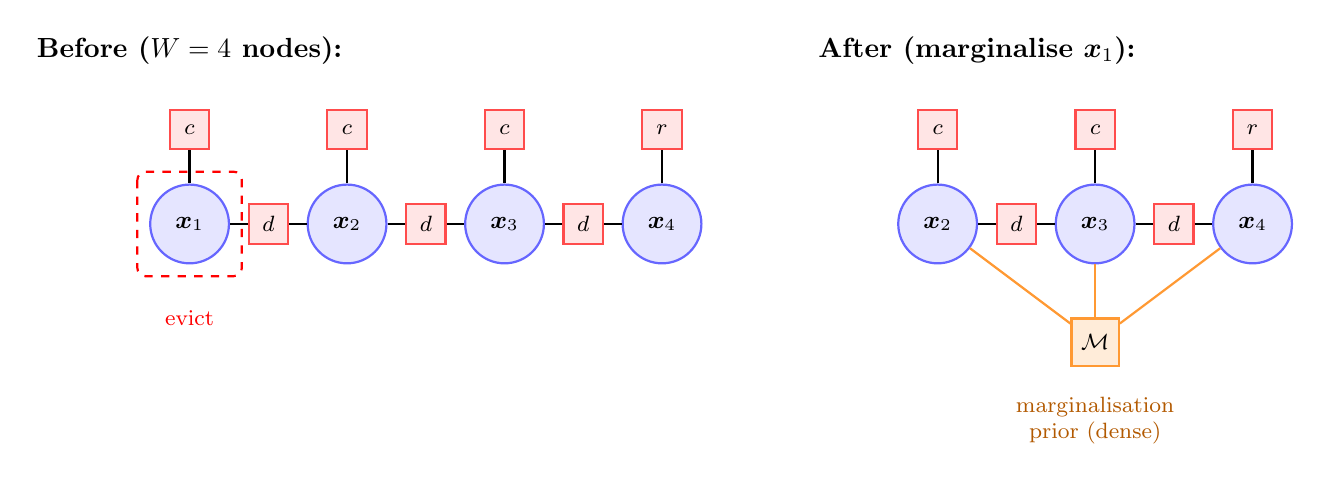
\begin{tikzpicture}[
    node distance=1.5cm,
    var/.style={circle, draw=blue!60, fill=blue!10, thick, minimum size=10mm, font=\small},
    factor/.style={rectangle, draw=red!70, fill=red!10, thick, minimum size=5mm, font=\footnotesize},
    marg/.style={rectangle, draw=orange!80, fill=orange!15, thick,
                 minimum width=6mm, minimum height=6mm, font=\footnotesize},
    >=Stealth
]
    % --- Before marginalization ---
    \node[font=\bfseries] at (0, 2.2) {Before ($W = 4$ nodes):};

    \node[var] (x1) at (0,0)  {$\bx_1$};
    \node[var] (x2) at (2,0)  {$\bx_2$};
    \node[var] (x3) at (4,0)  {$\bx_3$};
    \node[var] (x4) at (6,0)  {$\bx_4$};

    \node[factor] (f12) at (1,0) {$d$};
    \node[factor] (f23) at (3,0) {$d$};
    \node[factor] (f34) at (5,0) {$d$};

    \node[factor] (fc1) at (0, 1.2) {$c$};
    \node[factor] (fc2) at (2, 1.2) {$c$};
    \node[factor] (fc3) at (4, 1.2) {$c$};
    \node[factor] (fr4) at (6, 1.2) {$r$};

    \draw[thick] (x1) -- (f12) -- (x2);
    \draw[thick] (x2) -- (f23) -- (x3);
    \draw[thick] (x3) -- (f34) -- (x4);
    \draw[thick] (x1) -- (fc1);
    \draw[thick] (x2) -- (fc2);
    \draw[thick] (x3) -- (fc3);
    \draw[thick] (x4) -- (fr4);

    % highlight node to remove
    \draw[dashed, red, thick, rounded corners=3pt]
      ($(x1.north west)+(-0.3,0.3)$) rectangle ($(x1.south east)+(0.3,-0.3)$);
    \node[red, font=\footnotesize] at (0, -1.2) {evict};

    % --- After marginalization ---
    \node[font=\bfseries] at (10, 2.2) {After (marginalise $\bx_1$):};

    \node[var] (y2) at (9.5,0)  {$\bx_2$};
    \node[var] (y3) at (11.5,0) {$\bx_3$};
    \node[var] (y4) at (13.5,0) {$\bx_4$};

    \node[factor] (g23) at (10.5,0) {$d$};
    \node[factor] (g34) at (12.5,0) {$d$};

    \node[factor] (gc2) at (9.5, 1.2) {$c$};
    \node[factor] (gc3) at (11.5, 1.2) {$c$};
    \node[factor] (gr4) at (13.5, 1.2) {$r$};

    \draw[thick] (y2) -- (g23) -- (y3);
    \draw[thick] (y3) -- (g34) -- (y4);
    \draw[thick] (y2) -- (gc2);
    \draw[thick] (y3) -- (gc3);
    \draw[thick] (y4) -- (gr4);

    % Marg prior (dense, touching all remaining nodes)
    \node[marg] (mp) at (11.5, -1.5) {$\mathcal{M}$};
    \draw[thick, orange!80] (y2) -- (mp);
    \draw[thick, orange!80] (y3) -- (mp);
    \draw[thick, orange!80] (y4) -- (mp);

    \node[orange!70!black, font=\footnotesize, text width=3cm, align=center]
      at (11.5, -2.5) {marginalisation\\prior (dense)};

\end{tikzpicture}
\caption{Factor graph before and after marginalising node $\bx_1$.
         Factors: $d$ = dynamics, $c$ = camera, $r$ = radar.
         The marginalisation prior $\mathcal{M}$ is a \emph{dense} factor
         connecting all remaining nodes.}
\label{fig:marginalization}
\end{figure}

% ===========================================================================
\section{Properties of the Marginalization Prior}
\label{sec:properties}

\subsection{Information Preservation}

\begin{proposition}[No Information Loss]
  The marginalisation step preserves the Fisher information about the
  remaining variables $\bx_b$.  Specifically, the marginal information
  matrix $\bH_{\text{marg}}$ equals the exact marginal of the original
  joint distribution over $\bx_b$ (at the linearisation point).
\end{proposition}

\begin{proof}
  The joint Gaussian on $(\bx_a, \bx_b)$ has information matrix $\bH$
  and information vector $\bb$.  By the marginalisation formula for
  Gaussians in information form, the marginal over $\bx_b$ has
  information $\bH_{bb} - \bH_{ba}\bH_{aa}^{-1}\bH_{ab}$, which is
  exactly $\bH_{\text{marg}}$.
\end{proof}

\subsection{Fill-In: The Cost of Marginalization}

\begin{warnbox}[Sparsity Destruction]
  Even though the original Hessian is sparse (block-tridiagonal), the Schur
  complement \eqref{eq:H_schur} is generally \textbf{dense}.

  Reason: $\bH_{ba}$ has non-zeros only in the rows corresponding to $\bx_2$ (the
  node connected to $\bx_1$ by the dynamics factor).  However,
  $\bH_{aa}^{-1}\bH_{ab}$ propagates this coupling to all rows of $\bH_{bb}$.
  After repeated marginalisations, $\bH_{\text{marg}}$ is fully dense.
\end{warnbox}

This ``fill-in'' is the fundamental trade-off:
\begin{itemize}
  \item Larger $W$ $\Rightarrow$ more accurate (longer constraint history)
    but the dense marginalisation prior costs $\mathcal{O}((Wd)^2)$ storage
    and $\mathcal{O}((Wd)^3)$ solve.
  \item Smaller $W$ $\Rightarrow$ faster per step but less historical
    information.
\end{itemize}

\subsection{Linearisation Point Consistency}

\begin{warnbox}[First-Estimate Jacobian (FEJ) Caveat]
  The marginalisation prior was computed at a specific linearisation point
  $\hat{\bx}_b$.  If subsequent optimisation iterations significantly shift
  $\hat{\bx}_b$, the prior becomes inconsistent—it encodes the information
  matrix and gradient from the \emph{old} linearisation.

  In practice, this is handled by either:
  \begin{enumerate}
    \item \textbf{First-Estimate Jacobian (FEJ)}: always use the same
      linearisation point for the marginalised factors (used in OpenVINS).
    \item \textbf{Warm-starting}: ensure the Gauss--Newton converges well
      each step so the linearisation point changes minimally.
  \end{enumerate}

  In our implementation we use warm-starting (the previous solution initialises
  the next step), which works well when $W$ is large enough relative to the
  state dynamics.
\end{warnbox}

% ===========================================================================
\section{Factor Types in Our Problem}
\label{sec:factors}

We recall the four factor types and their residuals and Jacobians.  The
state per node is $\bx_k = [\bp_t^\top, \bv_t^\top]^\top \in \R^6$.

\subsection{Prior Factor}

\begin{equation}
  \br_{\text{prior}} = \bx_k - \bm{\mu}_0, \qquad
  \bJ = \bI_6, \qquad
  \bSigma = \bSigma_0.
\end{equation}

\subsection{Dynamics Factor (Constant Velocity)}

The prediction model:
\begin{equation}
  f(\bx_k) = \begin{bmatrix} \bp_t + \bv_t \Delta t \\ \bv_t \end{bmatrix},
\end{equation}
with residual and Jacobians:
\begin{align}
  \br &= \bx_{k+1} - f(\bx_k), \\
  \bJ_k &= -\bm{F}_k = -\begin{bmatrix} \bI_3 & \Delta t\,\bI_3 \\ \bm{0} & \bI_3 \end{bmatrix}, \qquad
  \bJ_{k+1} = \bI_6.
\end{align}

Process noise:
\begin{equation}
  \bSigma_{\text{dyn}} = \sigma_a^2
  \begin{bmatrix}
    \frac{\Delta t^4}{4}\bI_3 & \frac{\Delta t^3}{2}\bI_3 \\[3pt]
    \frac{\Delta t^3}{2}\bI_3 & \Delta t^2\,\bI_3
  \end{bmatrix}.
\end{equation}

\subsection{Camera Factor (Perspective Projection)}

Let $\bm{M} = \bR_{\text{b2c}}\,\bR_{\text{b2e}}^\top$.  The camera
computes the projection:
\begin{equation}
  \bp_{\text{cam}} = \bm{M}(\bp_t - \bp_i), \qquad
  h(\bx_k) = \begin{bmatrix} p_{\text{cam},x}/p_{\text{cam},z} \\
                               p_{\text{cam},y}/p_{\text{cam},z}
              \end{bmatrix}.
\end{equation}

Residual and Jacobian:
\begin{align}
  \br &= \bz_{\text{cam}} - h(\bx_k), \\
  \bJ &= -\frac{\partial h}{\partial \bp_t}\,\big[\bI_3 \;\; \bm{0}_{3\times3}\big]
       = -\begin{bmatrix}
           1/w & 0 & -u/w^2 \\
           0 & 1/w & -v/w^2
         \end{bmatrix}\,\bm{M}\,\big[\bI_3 \;\; \bm{0}\big],
\end{align}
where $(u, v, w) = \bp_{\text{cam}}$.

\subsection{Radar Factor (Direct Observation)}

\begin{equation}
  \br = \bz_{\text{radar}} - \bx_k, \qquad
  \bJ = -\bI_6.
\end{equation}

\subsection{Marginalisation Prior Factor}

After marginalisation produces $\bm{\mu}_{\text{marg}}$ and
$\bLambda_{\text{marg}} = \bm{L}\bm{L}^\top$:
\begin{equation}
  \br = \bx_b - \bm{\mu}_{\text{marg}}, \qquad
  \tilde{\br} = \bm{L}^{-1}\br, \qquad
  \tilde{\bJ} = \bm{L}^{-1}\,\frac{\partial \br}{\partial \bx_b} = \bm{L}^{-1}.
  \label{eq:marg_factor}
\end{equation}

Note that this is a \emph{dense} factor connecting all $(W-1)$ nodes.

% ===========================================================================
\section{Handling Measurement Delay in the Sliding Window}
\label{sec:delay}

Camera measurements arrive with a processing delay of $\tau$ seconds,
corresponding to $D = \lceil \tau / \Delta t \rceil$ nodes.  A measurement
captured at absolute node $k$ becomes available at node $k + D$.

\begin{keybox}[Delay Handling Rule]
  When processing step $k$: if the delayed camera measurement arrives
  (captured at node $k - D$) and $k - D$ is still inside the current
  window, attach the camera factor to node $k - D$.

  If $k - D$ is outside the window (\ie{} already marginalised), the
  measurement must be discarded—it cannot retroactively influence
  the evicted node.

  \textbf{Design rule:} choose $W \gg D$ to ensure delayed measurements
  are never wasted.
\end{keybox}

In our problem: $\Delta t = 0.1\,\text{s}$, $\tau = 80\,\text{ms}$,
so $D = 1$.  With $W = 15 \gg 1$, delayed measurements are always handled.

% ===========================================================================
\section{Algorithm Summary}
\label{sec:algorithm}

\begin{algorithm}[H]
\caption{Online Sliding-Window Factor Graph Optimisation}
\label{alg:swfgo}
\begin{algorithmic}[1]
\Require Window size $W$, max GN iterations $N_{\text{GN}}$, convergence threshold $\varepsilon$
\Ensure  Online state estimates $\{\hat{\bx}_k\}_{k=1}^{N}$

\State Initialise window with node $\bx_1$ and prior factor $\mathcal{N}(\bm{\mu}_0, \bSigma_0)$
\State $\mathcal{M} \leftarrow \varnothing$ \Comment{No marginalisation prior yet}

\For{$k = 2, 3, \ldots, N$}
  \If{window size $= W$}
    \State \textbf{Marginalise oldest node:}
    \State \hspace{1em} Build Hessian $\bH$ and gradient $\bb$ over current window
    \State \hspace{1em} Partition: $(\bH_{aa}, \bH_{ab}, \bH_{ba}, \bH_{bb})$ and $(\bb_a, \bb_b)$
    \State \hspace{1em} $\bH_{\text{marg}} \leftarrow \bH_{bb} - \bH_{ba}\,\bH_{aa}^{-1}\,\bH_{ab}$
    \State \hspace{1em} $\bb_{\text{marg}} \leftarrow \bb_b - \bH_{ba}\,\bH_{aa}^{-1}\,\bb_a$
    \State \hspace{1em} $\bm{\mu}_{\text{marg}} \leftarrow \hat{\bx}_b + \bH_{\text{marg}}^{-1}\,\bb_{\text{marg}}$
    \State \hspace{1em} $\bm{L}_{\text{marg}} \leftarrow \text{chol}(\bH_{\text{marg}})$
    \State \hspace{1em} Store $\mathcal{M} = (\bm{\mu}_{\text{marg}}, \bm{L}_{\text{marg}}^{-1})$
    \State \hspace{1em} Remove oldest node and prune its factors
  \EndIf

  \State Add node $\bx_k$ (initialised by dead-reckoning from $\hat{\bx}_{k-1}$)
  \State Add dynamics factor $\bx_{k-1} \to \bx_k$
  \If{camera measurement at node $k - D$ is available \textbf{and} $k-D$ is in window}
    \State Add camera factor on node $k - D$
  \EndIf
  \If{radar measurement at node $k$ is available}
    \State Add radar factor on node $k$
  \EndIf

  \State \textbf{Optimise:} Run Gauss--Newton for at most $N_{\text{GN}}$ iterations:
  \For{$\ell = 1, \ldots, N_{\text{GN}}$}
    \State Build $\tilde{\bJ}$, $\tilde{\br}$ from all active factors $+$ $\mathcal{M}$
    \State $\bH \leftarrow \tilde{\bJ}^\top\tilde{\bJ}$;
           $\quad \bb \leftarrow -\tilde{\bJ}^\top\tilde{\br}$
    \State $\delta\bx \leftarrow (\bH + \lambda\bI)^{-1}\,\bb$
    \State $\hat{\bx} \leftarrow \hat{\bx} + \delta\bx$
    \If{$\|\delta\bx\| < \varepsilon$}
      \State \textbf{break}
    \EndIf
  \EndFor

  \State Store estimate $\hat{\bx}_k$ and marginal covariance $[\bH^{-1}]_{kk}$
\EndFor
\end{algorithmic}
\end{algorithm}

% ===========================================================================
\section{Complexity Analysis}
\label{sec:complexity}

\begin{table}[h!]
\centering
\begin{tabular}{lcc}
\toprule
\textbf{Operation} & \textbf{Batch FGO} & \textbf{SW-FGO (per step)} \\
\midrule
Unknown dimension   & $Nd$               & $Wd$ \\
Hessian assembly    & $\mathcal{O}(Nd^2)$  & $\mathcal{O}(Wd^2)$ \\
Hessian solve       & $\mathcal{O}((Nd)^3)^\dagger$
                    & $\mathcal{O}((Wd)^3)$ \\
Schur complement    & ---                & $\mathcal{O}(d^3 + (Wd)^2 d)$ \\
Memory              & $\mathcal{O}(Nd)$  & $\mathcal{O}(Wd + (Wd)^2)^\ddagger$ \\
\bottomrule
\end{tabular}
\caption{Complexity comparison.  $^\dagger$Exploiting banded structure
  reduces to $\mathcal{O}(Nd^2)$, but this is an asymptotic lower bound.
  $^\ddagger$The $(Wd)^2$ term is due to the dense marginalisation prior.}
\label{tab:complexity}
\end{table}

For our problem: $d = 6$, $N = 301$, $W = 15$.  The batch system has
$301 \times 6 = 1806$ unknowns; the window system has $15 \times 6 = 90$
unknowns per step—a $20\times$ reduction.

% ===========================================================================
\section{Connection to the Kalman Filter}
\label{sec:kalman}

The sliding-window FGO with $W = 1$ (single node) is equivalent
to the Extended Kalman Filter:
\begin{itemize}
  \item The marginalisation prior on $\bx_k$ is the \emph{predicted}
    state distribution $\mathcal{N}(\hat{\bx}_{k|k-1}, \bSigma_{k|k-1})$.
  \item Adding a measurement factor and optimising (one GN step)
    is the Kalman \emph{update} step.
  \item Marginalising $\bx_k$ and predicting $\bx_{k+1}$ is the
    \emph{prediction} step.
\end{itemize}

With $W > 1$, the sliding-window re-optimises past states that are still
in the window—this is a form of \textbf{fixed-lag smoothing} that
the standard EKF cannot perform.

\begin{table}[h!]
\centering
\begin{tabular}{lccc}
\toprule
& \textbf{EKF} & \textbf{SW-FGO} & \textbf{Batch FGO} \\
\midrule
Window size         & $W = 1$   & $1 < W \ll N$  & $W = N$ \\
Past-state refinement & No       & Yes ($W$ nodes) & Yes (all) \\
Linearisation quality & Single point & $N_{\text{GN}}$ re-iterations & Full convergence \\
Info from history   & Exact (propagated) & Approx.\ (Schur prior) & Exact \\
\bottomrule
\end{tabular}
\caption{Spectrum of estimators: the sliding-window is a tuneable
         interpolation between the EKF ($W=1$) and batch ($W=N$).}
\end{table}

% ===========================================================================
\section{Numerical Example: Hessian Structure}
\label{sec:example}

Consider a window with $W = 4$ nodes ($d = 6$, total dim = 24).
Before marginalisation, the Hessian has block-tridiagonal structure from the
dynamics plus diagonal contributions from measurements:

\begin{equation}
  \bH = \begin{bmatrix}
    \bH_{11}^{\text{dyn+cam+marg}} & \bH_{12}^{\text{dyn}} & & \\
    \bH_{21}^{\text{dyn}} & \bH_{22}^{\text{dyn+cam}} & \bH_{23}^{\text{dyn}} & \\
    & \bH_{32}^{\text{dyn}} & \bH_{33}^{\text{dyn+cam}} & \bH_{34}^{\text{dyn}} \\
    & & \bH_{43}^{\text{dyn}} & \bH_{44}^{\text{dyn+rad}}
  \end{bmatrix}.
\end{equation}

After marginalising node 1, the Schur complement creates fill-in:
\begin{equation}
  \bH_{\text{marg}} = \begin{bmatrix}
    \bH_{22}' & \bH_{23}^{\text{dyn}} & \\
    \bH_{32}^{\text{dyn}} & \bH_{33}' & \bH_{34}^{\text{dyn}} \\
    & \bH_{43}^{\text{dyn}} & \bH_{44}'
  \end{bmatrix}
  + \underbrace{\text{dense fill-in from marg}}_{\text{no longer sparse!}}.
\end{equation}

In practice, the fill-in primarily affects the block rows/columns
connected to node 2 (the direct neighbour of the evicted node 1).
After multiple marginalisations, the accumulated prior becomes fully
dense.

% ===========================================================================
\section{Summary}
\label{sec:summary}

\begin{enumerate}
  \item \textbf{Batch FGO} solves the full problem at once—optimal but
    grows without bound.
  \item \textbf{Sliding-window FGO} fixes the window size to $W$ nodes,
    yielding bounded-complexity online estimation.
  \item The \textbf{Schur complement} is the mathematical tool for
    evicting old nodes:
    \[
      \bH_{\text{marg}} = \bH_{bb} - \bH_{ba}\,\bH_{aa}^{-1}\,\bH_{ab},
      \qquad
      \bb_{\text{marg}} = \bb_b - \bH_{ba}\,\bH_{aa}^{-1}\,\bb_a.
    \]
  \item The marginalised prior is \textbf{lossless at the linearisation
    point}—it encodes the exact Fisher information from all evicted
    factors.
  \item The trade-off: the prior is \textbf{dense} (destroys sparsity) and
    \textbf{linearisation-point dependent}.
  \item Measurement delays are handled by attaching factors to past nodes
    that are still inside the window.
  \item The sliding-window can be viewed as a smooth interpolation between
    an EKF ($W = 1$) and batch FGO ($W = N$).
\end{enumerate}

% ===========================================================================
\begin{thebibliography}{9}

\bibitem{kaess2008}
  M.~Kaess, A.~Ranganathan, and F.~Dellaert,
  ``iSAM: Incremental smoothing and mapping,''
  \emph{IEEE Trans.\ Robotics}, vol.~24, no.~6, pp.~1365--1378, 2008.

\bibitem{mourikis2007}
  A.~I.~Mourikis and S.~I.~Roumeliotis,
  ``A multi-state constraint Kalman filter for vision-aided inertial navigation,''
  in \emph{Proc.\ IEEE ICRA}, 2007, pp.~3565--3572.

\bibitem{leutenegger2015}
  S.~Leutenegger \emph{et al.},
  ``Keyframe-based visual-inertial odometry using nonlinear optimization,''
  \emph{Int.\ J.\ Robotics Research}, vol.~34, no.~3, pp.~314--334, 2015.

\bibitem{qin2018}
  T.~Qin, P.~Li, and S.~Shen,
  ``VINS-Mono: A robust and versatile monocular visual-inertial state estimator,''
  \emph{IEEE Trans.\ Robotics}, vol.~34, no.~4, pp.~1004--1020, 2018.

\bibitem{geneva2020}
  P.~Geneva \emph{et al.},
  ``OpenVINS: A research platform for visual-inertial state estimation,''
  in \emph{Proc.\ IEEE ICRA}, 2020, pp.~4666--4672.

\bibitem{dellaert2017}
  F.~Dellaert and M.~Kaess,
  ``Factor graphs for robot perception,''
  \emph{Foundations and Trends in Robotics}, vol.~6, no.~1--2, pp.~1--139, 2017.

\bibitem{sibley2010}
  G.~Sibley, L.~Matthies, and G.~Sukhatme,
  ``Sliding window filter with application to planetary landing,''
  \emph{J.\ Field Robotics}, vol.~27, no.~5, pp.~587--608, 2010.

\end{thebibliography}

\end{document}
